%%=============================================================================
%% Conclusie
%%=============================================================================

\chapter{Resultaten}
\label{ch:resultaten}

\section{Intentherkenning zonder het gebruik van entities}
\label{intent}

Bij het eerste en belangrijkste experiment werden geen entities gebruikt in de dataset en werd puur beoordeeld op intentherkenning. Elk platform is uitgebreid getest door middel van 5-fold cross validation. Elk platform is dus vijf keer gebouwd, getraind en getest geweest om een objectief beeld te krijgen van hoe goed elk platform de juiste intent kan herkennen bij een specifieke input. Van alle resultaten werden confusion matrices opgesteld en werden de precision, recall en F-scores berekend.

\begin{figure}[H]
    \label{fig:confusion-matrix-watson}
    \centering
    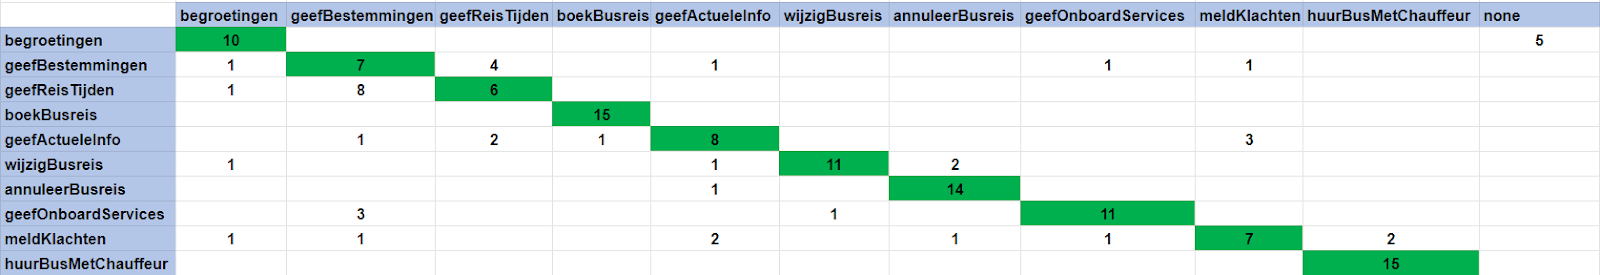
\includegraphics[width=\textwidth]{confusion-matrix-watson}
    \caption{Algemene confusion matrix intentherkenning zonder entities van IBM Watson}
\end{figure}

\begin{figure}[H]
    \label{fig:confusion-matrix-luis}
    \centering
    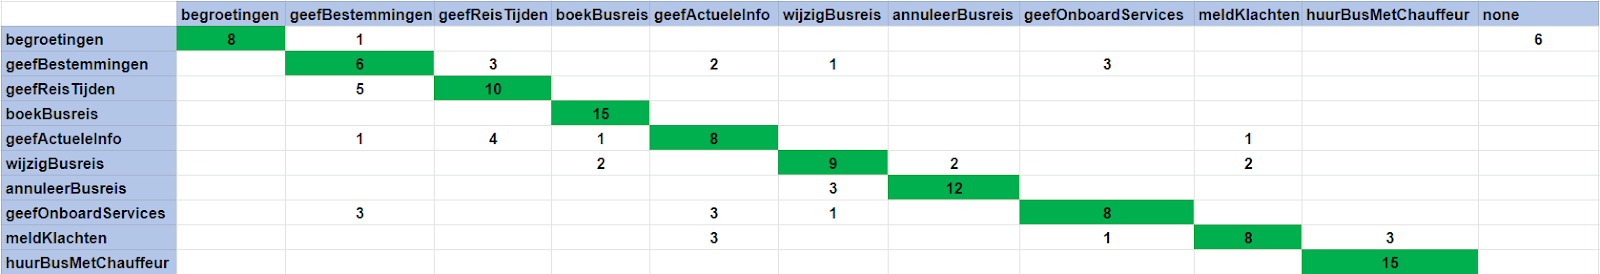
\includegraphics[width=\textwidth]{confusion-matrix-luis}
    \caption{Algemene confusion matrix intentherkenning zonder entities van LUIS}
\end{figure}

\begin{figure}[H]
    \label{fig:confusion-matrix-rasa}
    \centering
    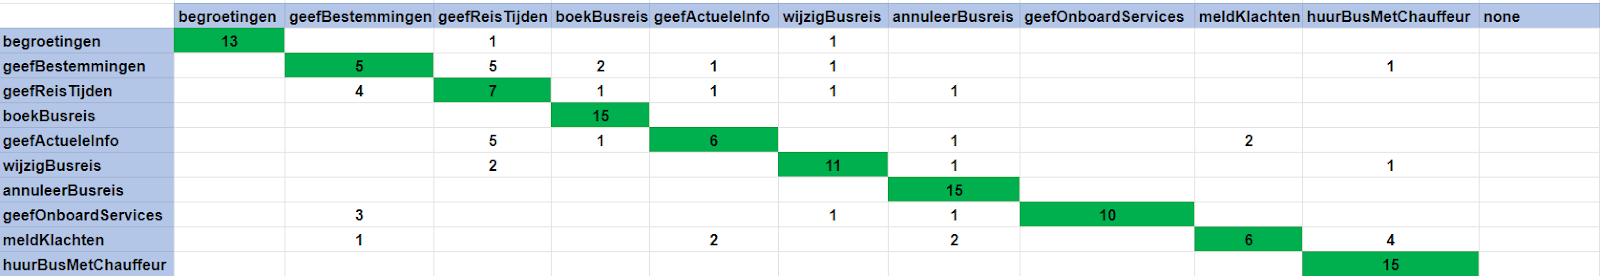
\includegraphics[width=\textwidth]{confusion-matrix-rasa}
    \caption{Algemene confusion matrix intentherkenning zonder entities van Rasa}
\end{figure}

\begin{figure}[H]
    \label{fig:confusion-matrix-wit}
    \centering
    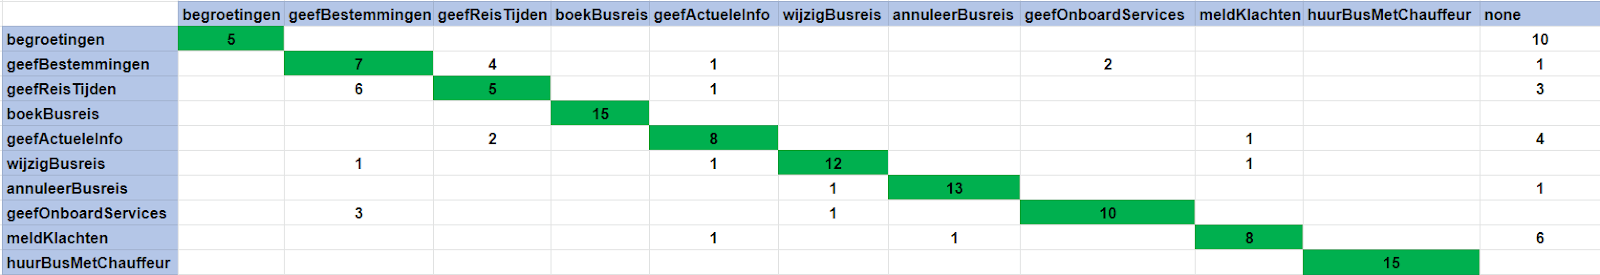
\includegraphics[width=\textwidth]{confusion-matrix-wit}
    \caption{Algemene confusion matrix intentherkenning zonder entities van Wit.ai}
\end{figure}

\begin{figure}[H]
    \label{fig:confusion-matrix-dialogflow}
    \centering
    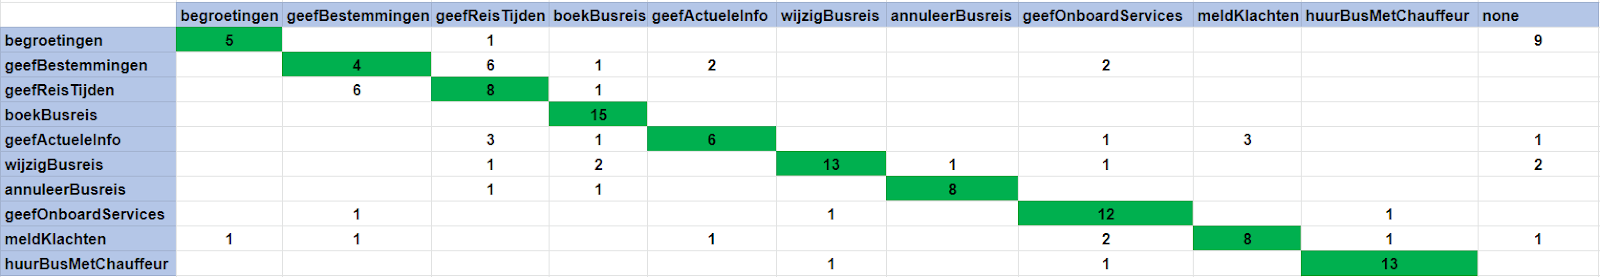
\includegraphics[width=\textwidth]{confusion-matrix-dialogflow}
    \caption{Algemene confusion matrix intentherkenning zonder entities van Dialogflow}
\end{figure}

\subsection{Onderlinge vergelijking}
\label{subsec:intent-onderling}

Op het eerste zicht valt het op dat er geen platform veel sterker presteert dan een andere. De gemiddelde resulaten van Wit.ai zijn de beste, met eerstvolgende achtervolgers IBM Watson en Rasa. Die resultaten verschillen telkens maar één procent, dus dat is praktisch verwaarloosbaar. Dialogflow presteert wel duidelijk minder dan de andere vier platformen. Daarnaast is het ook opvallend dat er duidelijke verschillen zitten in de gemiddelde resultaten van de cycli zelf. De resultaten van cyclus twee liggen duidelijk hoger dan de andere gemiddelden en cyclus vijf scoort duidelijk het slechtst. Dat is volledig te wijten aan toeval van hoe het algoritme de dataset heeft verdeeld tijdens de uitvoering van cross validation. Als laatste is het ook belangrijk om stil te staan bij de F-scores van de individuele intents, daarbij valt het op dat bepaalde intents opmerkelijk slecht scoren in vergelijking met andere. Dit komt omdat de platformen de intents, die slechter scoorden, vaak ging verwisselen met elkaar. Dat kan ook duidelijk worden vastgesteld in de verschillende confusion matrices.

Om de precision, recall en F-score van 1 cyclus te berekenen, moeten we een aantal zaken van de intents optellen met elkaar vanuit de respectievelijke confusion matrices:
\begin{itemize}
    \item Het aantal keer dat elke intent juist werd voorspeld, dit noemen we de true positives (TP).
    \item Het aantal keer dat elke intent werd voorspeld, maar eigenlijk niet verwacht werd, dit noemen we de false negatives (FN).
    \item Het aantal keer dat elke intent werd verwacht, maar niet juist werd voorspeld, dit noemen we de false positives (FP).
\end{itemize}
Daaruit kunnen we de volgende metrieken juist berekenen:
\begin{itemize}
    \item $Precision = \frac{TP}{TP + FP}\\$
    \item $Recall = \frac{TP}{TP + FN}\\$
    \item F-score $= 2 * \frac{precision*recall}{precision+recall}\\$
\end{itemize}

\begin{figure}[H]
    \label{fig:cycle-2-calc-wit}
    \centering
    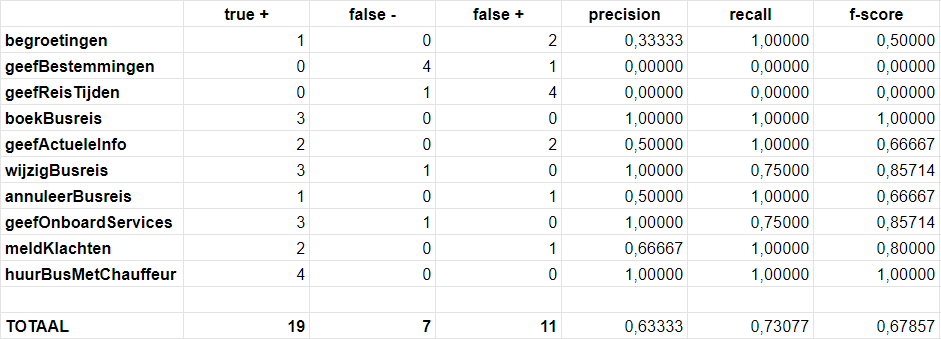
\includegraphics[width=\textwidth]{cycle-2-calc-wit}
    \caption{Berekeningen om de F-score van cyclus 2 van Wit.ai te bekomen bij intentherkenning zonder entities}
\end{figure}

\begin{center}
    \begin{longtable}{| l | l | l | l | l |  l | l | l |}
        \hline
        \textbf{Platform} & \textbf{Cyclus 1} & \textbf{Cyclus 2} & \textbf{Cyclus 3} & \textbf{Cyclus 4} & \textbf{Cyclus 5} & \textbf{Totaal} \\ \hline
         \textbf{Wit.ai} & 0,61818 & 0,67857 & 1,00000 & 0,67925 & 0,54902 & \textbf{0,71273 $\pm$ 0,15508} \\ \hline  
        \textbf{IBM Watson} & 0,70000 & 0,76667 & 0,67797 & 0,81356 & 0,56140 & \textbf{0,70508 $\pm$ 0,08508} \\ \hline 
         \textbf{Rasa} & 0,66667 & 0,76667 & 0,66667 & 0,70000 & 0,63333 & \textbf{0,68667 $\pm$ 0,04522} \\ \hline 
        \textbf{LUIS} & 0,61017 & 0,76667 & 0,64407 & 0,76667 & 0,57143 & \textbf{0,67347 $\pm$ 0,08080} \\ \hline           
        \textbf{Dialogflow} & 0,64407 & 0,71429 & 0,67797 & 0,60714 & 0,56140 & \textbf{0,64111 $\pm$ 0,05335} \\ \hline  
        \textbf{Totaal} & \textbf{0,64782} & \textbf{0,73857} & \textbf{0,67797} & \textbf{0,60714} & \textbf{0,5614} &    \\
        & \textbf{$\pm$ 0,03283} & \textbf{$\pm$ 0,03622} & \textbf{$\pm$ 0,13391} & \textbf{$\pm$ 0,07142} & \textbf{$\pm$ 0,02986} &    \\ \hline
        \caption{Tabel met F-scores per platform voor intentherkenning zonder entities}                                    
    \end{longtable}
    \label{tbl:results-intent-no-entity}
\end{center}

\begin{figure}[H]
    \label{fig:chart-intent-no-entity}
    \centering
    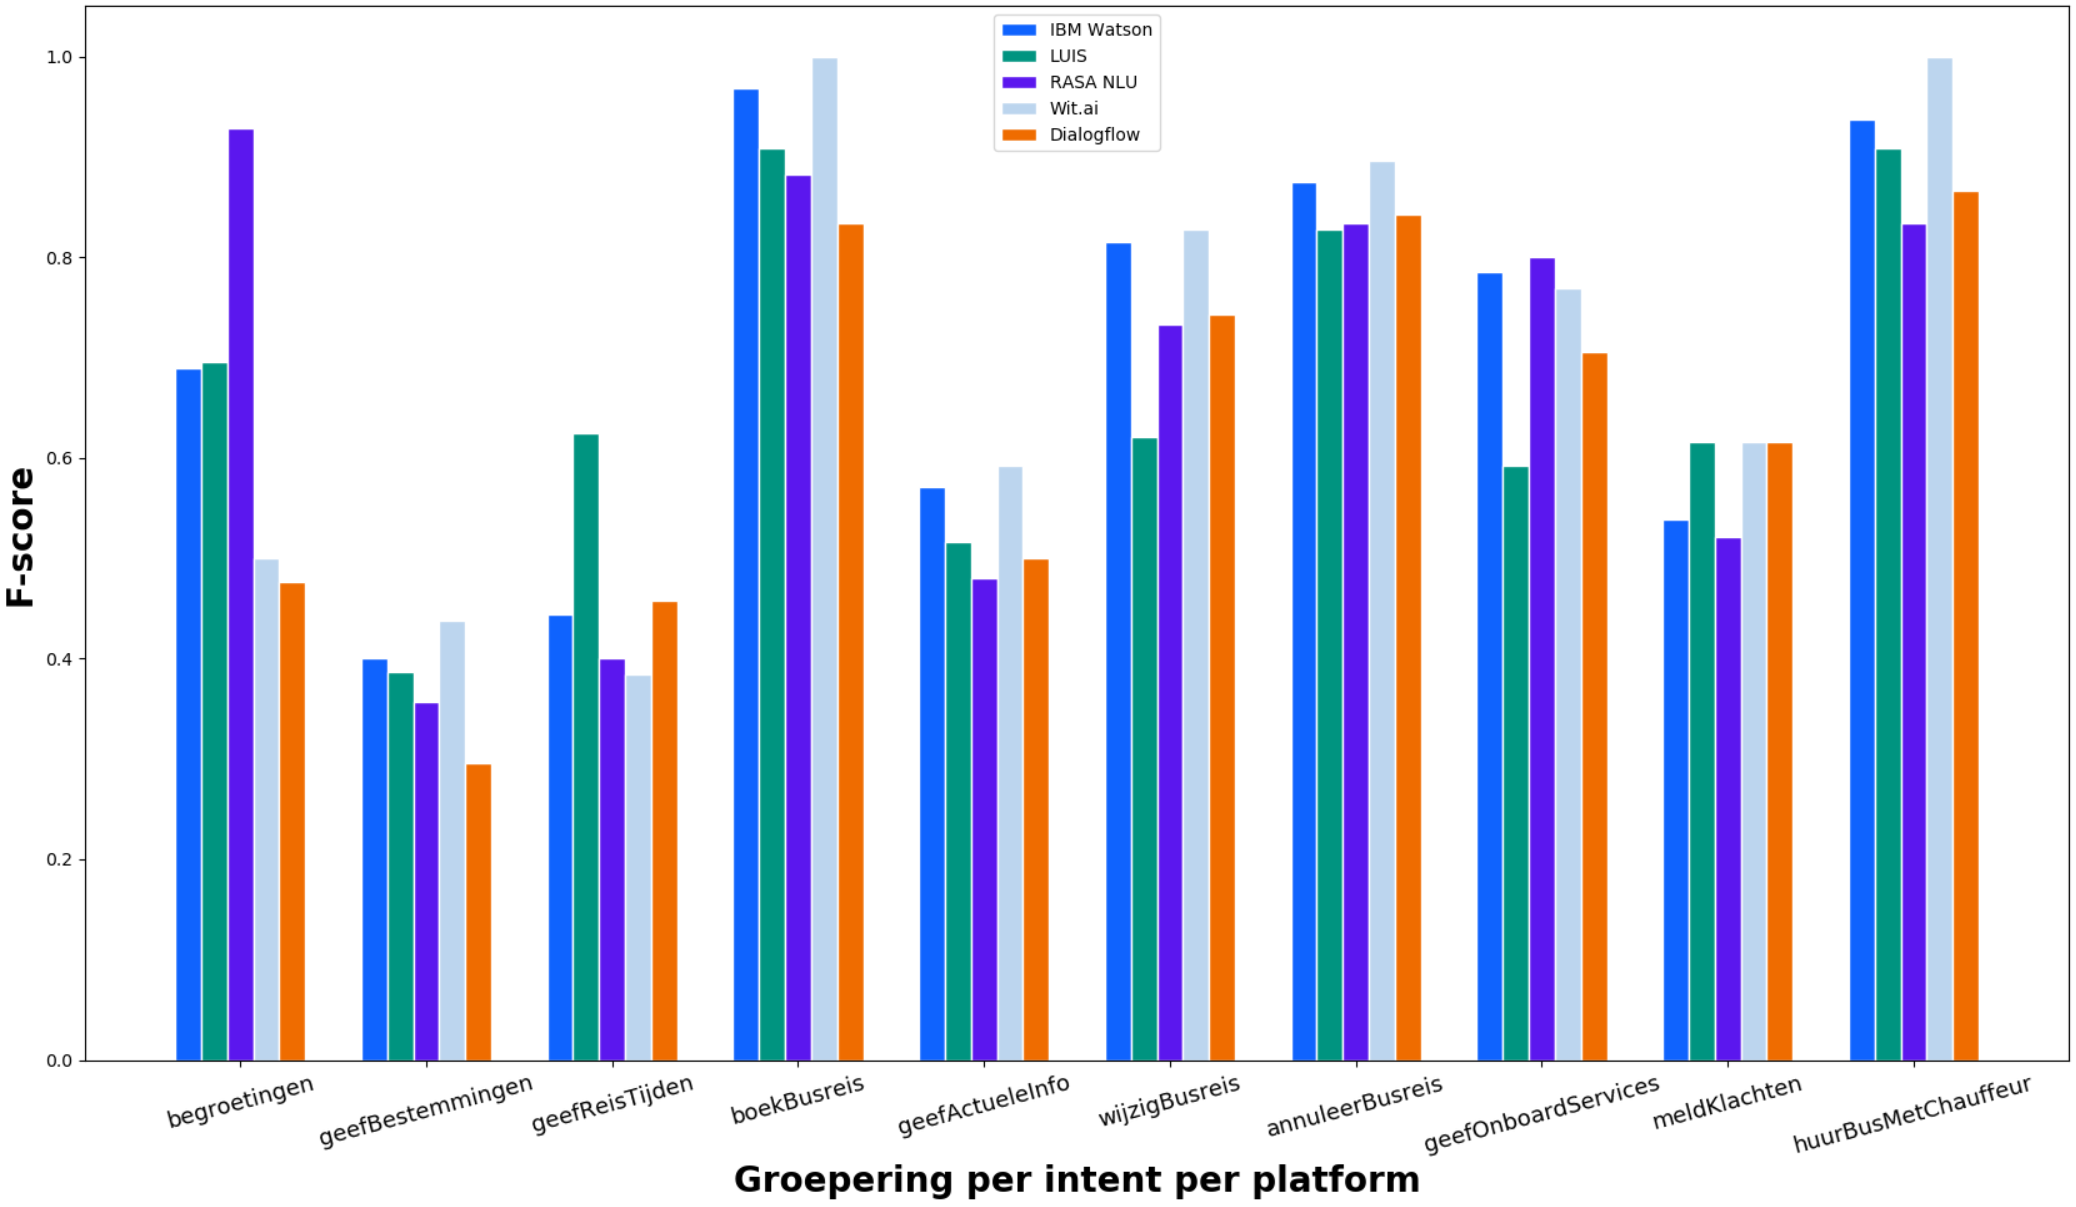
\includegraphics[width=\textwidth]{chart-intent}
    \caption{Grafiek die de F-scores per intent per platform visualiseert voor intentherkenning zonder entities}
\end{figure}

\section{Intent-en-entityherkenning}

Bij het tweede experiment werd gekeken naar hoe goed de platformen entities kunnen afleiden uit de input en hoe het zit met intentherkenning bij het gebruik van entities. Daarbij werd, in tegenstelling tot het eerste experiment, maar één iteratie uitgevoerd. Dit komt omdat het eerste experiment het hoofdexperiment is van deze bachproef en hier is dus extra aandacht aan besteed. 5-fold cross validation uitvoeren neemt erg veel tijd in beslag, daarom dat er een keuze moest worden gemaakt. Voor dit experiment werd de dataset door middel van een algoritme verdeeld in twee delen, een dataset om te trainen (80\% van de data) en een dataset om te valideren (20\% van de data). Alle platformen werden getraind en gevalideerd op een manier dat ze nu wel entities bevatten. Uit de resultaten valt het meteen op dat de F-scores gemiddeld hoger liggen dan bij het eerste experiment. Dit moet met een korrel zout genomen worden, doordat er maar één iteratie is uitgevoerd en omdat er nieuwe train-en-test datasets gegenereerd zijn. Dus door toeval kunnen er ‘makkelijkere’ testzinnen gebruikt zijn. Bij deze resultaten is het duidelijk dat IBM Watson de betere resultaten kan voorleggen en dat het in tegenstelling tot het vorige experiment Wit.ai is die het slechtst scoort.


\begin{center}
    \begin{longtable}{| l | l |}
        \hline
        \textbf{Platform} & \textbf{F-score} \\ \hline
        \textbf{IBM Watson} & 0,80000 \\ \hline  
        \textbf{LUIS} & 0,74576 \\ \hline  
        \textbf{Rasa} & 0,70000 \\ \hline  
        \textbf{Wit.ai} & 0,65455  \\ \hline  
        \textbf{Dialogflow} & 0,72414 \\ \hline  
        \caption{Tabel met F-scores per platform voor intentherkenning met het gebruik van entities}                                    
    \end{longtable}
    \label{tbl:results-intent-entity}
\end{center}

\subsection{Entityherkenning}

Het belangrijkste deel van dit experiment is het valideren van de entitiyherkenning, hierbij werd gebruik gemaakt van zowel systeementiteiten, als van zelfgedefinieerde entiteiten. De entiteiten die geanalyseerd zullen worden zijn beschreven in sectie \ref{sec:dataset}. IBM Watson heeft tot op heden geen systeementiteit die locaties kan herkennen in het Nederlands, dat kon dus niet beoordeeld worden. Bij LUIS is het problematischer, daar zijn er geen systeementiteiten in het Nederlands voor het herkennen van locaties, datums en tijdstippen, dit bestond vroeger wel, maar dat is stopgezet in december 2018. Er is een alternatief dat op basis van machine learning alles zou herkennen, maar dit bleek niet vlot te werken en heeft geen resultaten opgeleverd. Door deze tekorten liggen de scores van beide platformen voor entityherkenning een stuk lager, maar op de andere entities scoren ze wel aanzienlijk goed. 

Uit de resultaten valt het meteen op dat Wit.ai de grote winnaar is bij het herkennen van parameterwaarden, dit is ook duidelijk te zien in de grafiek waarbij de scores per entity worden voorgesteld. Wit.ai scoort op elke entiteit minstens even goed of een stuk beter dan zijn concurrenten.

\begin{center}
    \begin{longtable}{| l | l |}
        \hline
        \textbf{Platform} & \textbf{F-score} \\ \hline
        \textbf{IBM Watson} & 0,62687 \\ \hline  
        \textbf{LUIS} & 0,26923 \\ \hline  
        \textbf{Rasa} & 0,79452 \\ \hline  
        \textbf{Wit.ai} & 0,95556  \\ \hline  
        \textbf{Dialogflow} & 0,83544 \\ \hline  
        \caption{Tabel met F-scores per platform voor entityherkenning}                                    
    \end{longtable}
    \label{tbl:results-entity}
\end{center}

\begin{figure}[H]
    \label{fig:chart-entity}
    \centering
    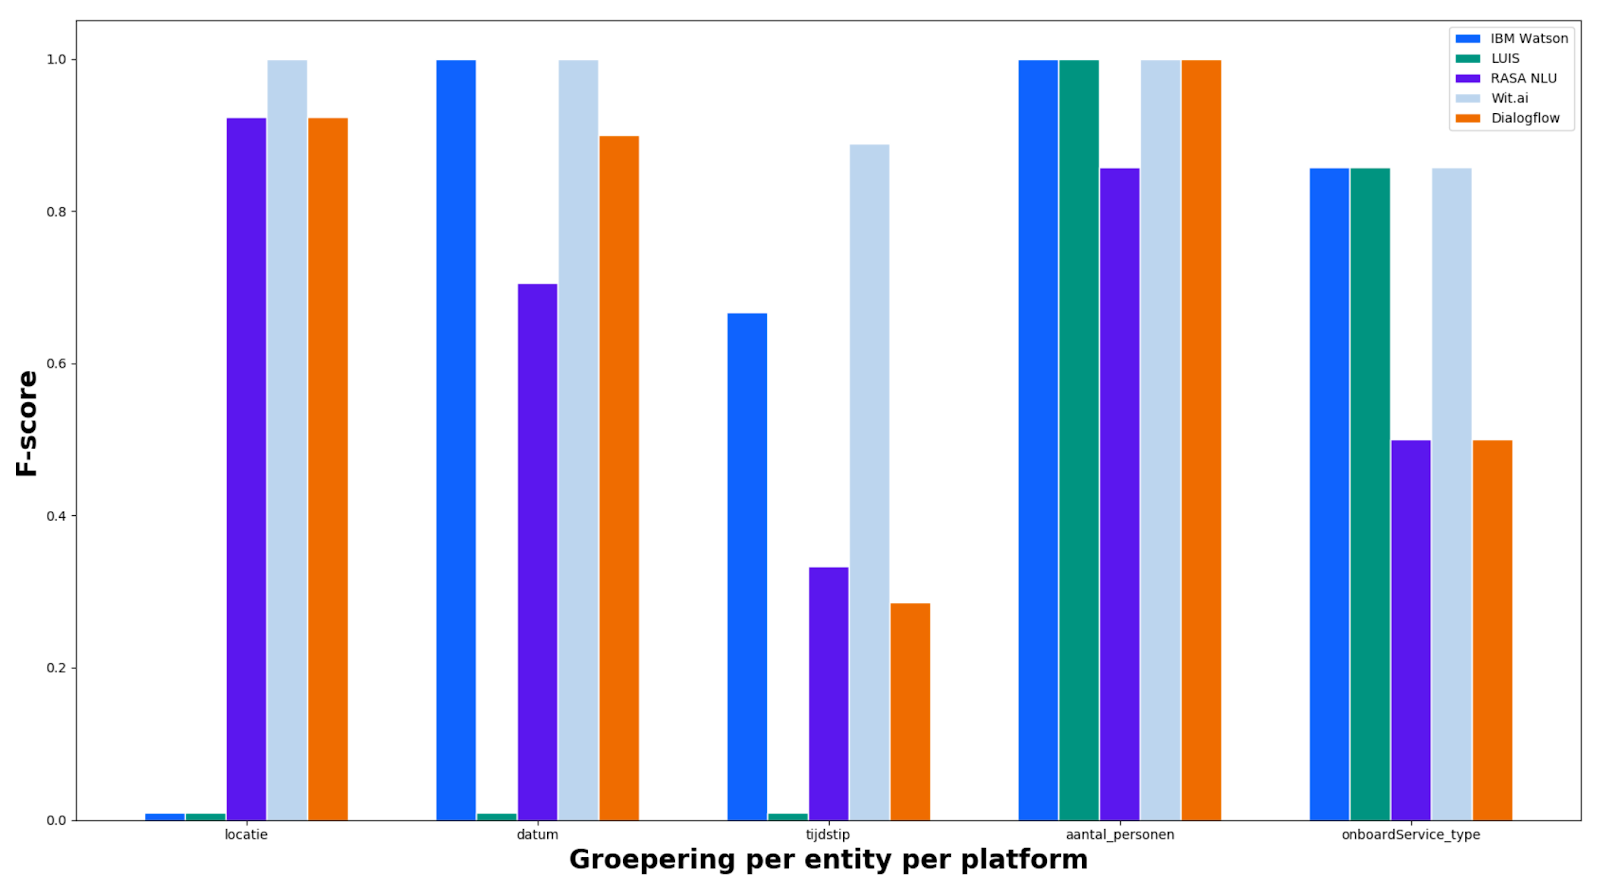
\includegraphics[width=\textwidth]{chart-entity}
    \caption{Grafiek die de F-scores per entity per platform visualiseert}
\end{figure}

\section{Invloed van spelling op Intent-en-entityherkenning}

Als laatste werd er gekeken naar hoe goed de platformen intents en entities kunnen herkennen als er een aanzienlijke hoeveelheid taalfouten in staan. Dit is delicaat om te valideren, omdat we met te kleine datasets werken om een volledig beeld te kunnen geven. Het is daarom ook slechts een indicatie van hoe goed de platformen hiermee omgaan. Er werden zowel taalfouten in intents als in entities beoordeeld. Opnieuw werd er slechts één iteratie uitgevoerd met dezelfde reden als voorgaand experiment. Er werd gebruik gemaakt van dezelfde datasets als bij het vorige experiment om een vergelijking te kunnen maken.

Om taalfouten te valideren, werden er manueel een aanzienlijke hoeveelheid fouten toegevoegd in de dataset. Daarbij zitten de fouten vooral in:
\begin{itemize}
    \item werkwoorden 
    \item grammatica (bijvoorbeeld dialect en afkortingen)
    \item locaties en datums
\end{itemize}

Wat opvalt is dat de resultaten van intentherkenning duidelijk lager liggen als er spellingsfouten gemaakt worden. Daarbij blijft IBM Watson wel het beste scoren. De sterkste daling in resultaten kunnen we vinden bij Dialogflow, die 22\% lager scoort.

\begin{center}
    \begin{longtable}{| l | l |}
        \hline
        \textbf{Platform} & \textbf{F-score} \\ \hline
        \textbf{IBM Watson} & 0,67797 \\ \hline  
        \textbf{LUIS} & 0,61017 \\ \hline  
        \textbf{Rasa} & 0,63333 \\ \hline  
        \textbf{Wit.ai} & 0,54545  \\ \hline  
        \textbf{Dialogflow} & 0,50000 \\ \hline  
        \caption{Tabel met F-scores per platform voor intentherkenning bij het gebruik van spellingsfouten}                                    
    \end{longtable}
    \label{tbl:results-intent-spelling}
\end{center}

\subsection{Entityherkenning}

Opnieuw werden ook de prestaties van entityherkenning in acht genomen, daarbij gelden dezelfde limitaties als vorig experiment van IBM Watson en LUIS. Hierbij liggen de resultaten ook gemiddeld lager dan voordien. De grote winnaar blijft immers wel Wit.ai, die nog steeds heel erg goede resultaten kan voorleggen. De grootste dalers zijn Rasa en Dialogflow die respectievelijk dalen met 34\% en 27\%.

\begin{center}
    \begin{longtable}{| l | l |}
        \hline
        \textbf{Platform} & \textbf{F-score} \\ \hline
        \textbf{IBM Watson} & 0,56250 \\ \hline  
        \textbf{LUIS} & 0,20000 \\ \hline  
        \textbf{Rasa} & 0,44828 \\ \hline  
        \textbf{Wit.ai} & 0,81013  \\ \hline  
        \textbf{Dialogflow} & 0,57143 \\ \hline  
        \caption{Tabel met F-scores per platform voor entityherkenning bij spellingsfouten}                                    
    \end{longtable}
    \label{tbl:results-entity-spelling}
\end{center}

\begin{figure}[H]
    \label{fig:chart-entity-spelling}
    \centering
    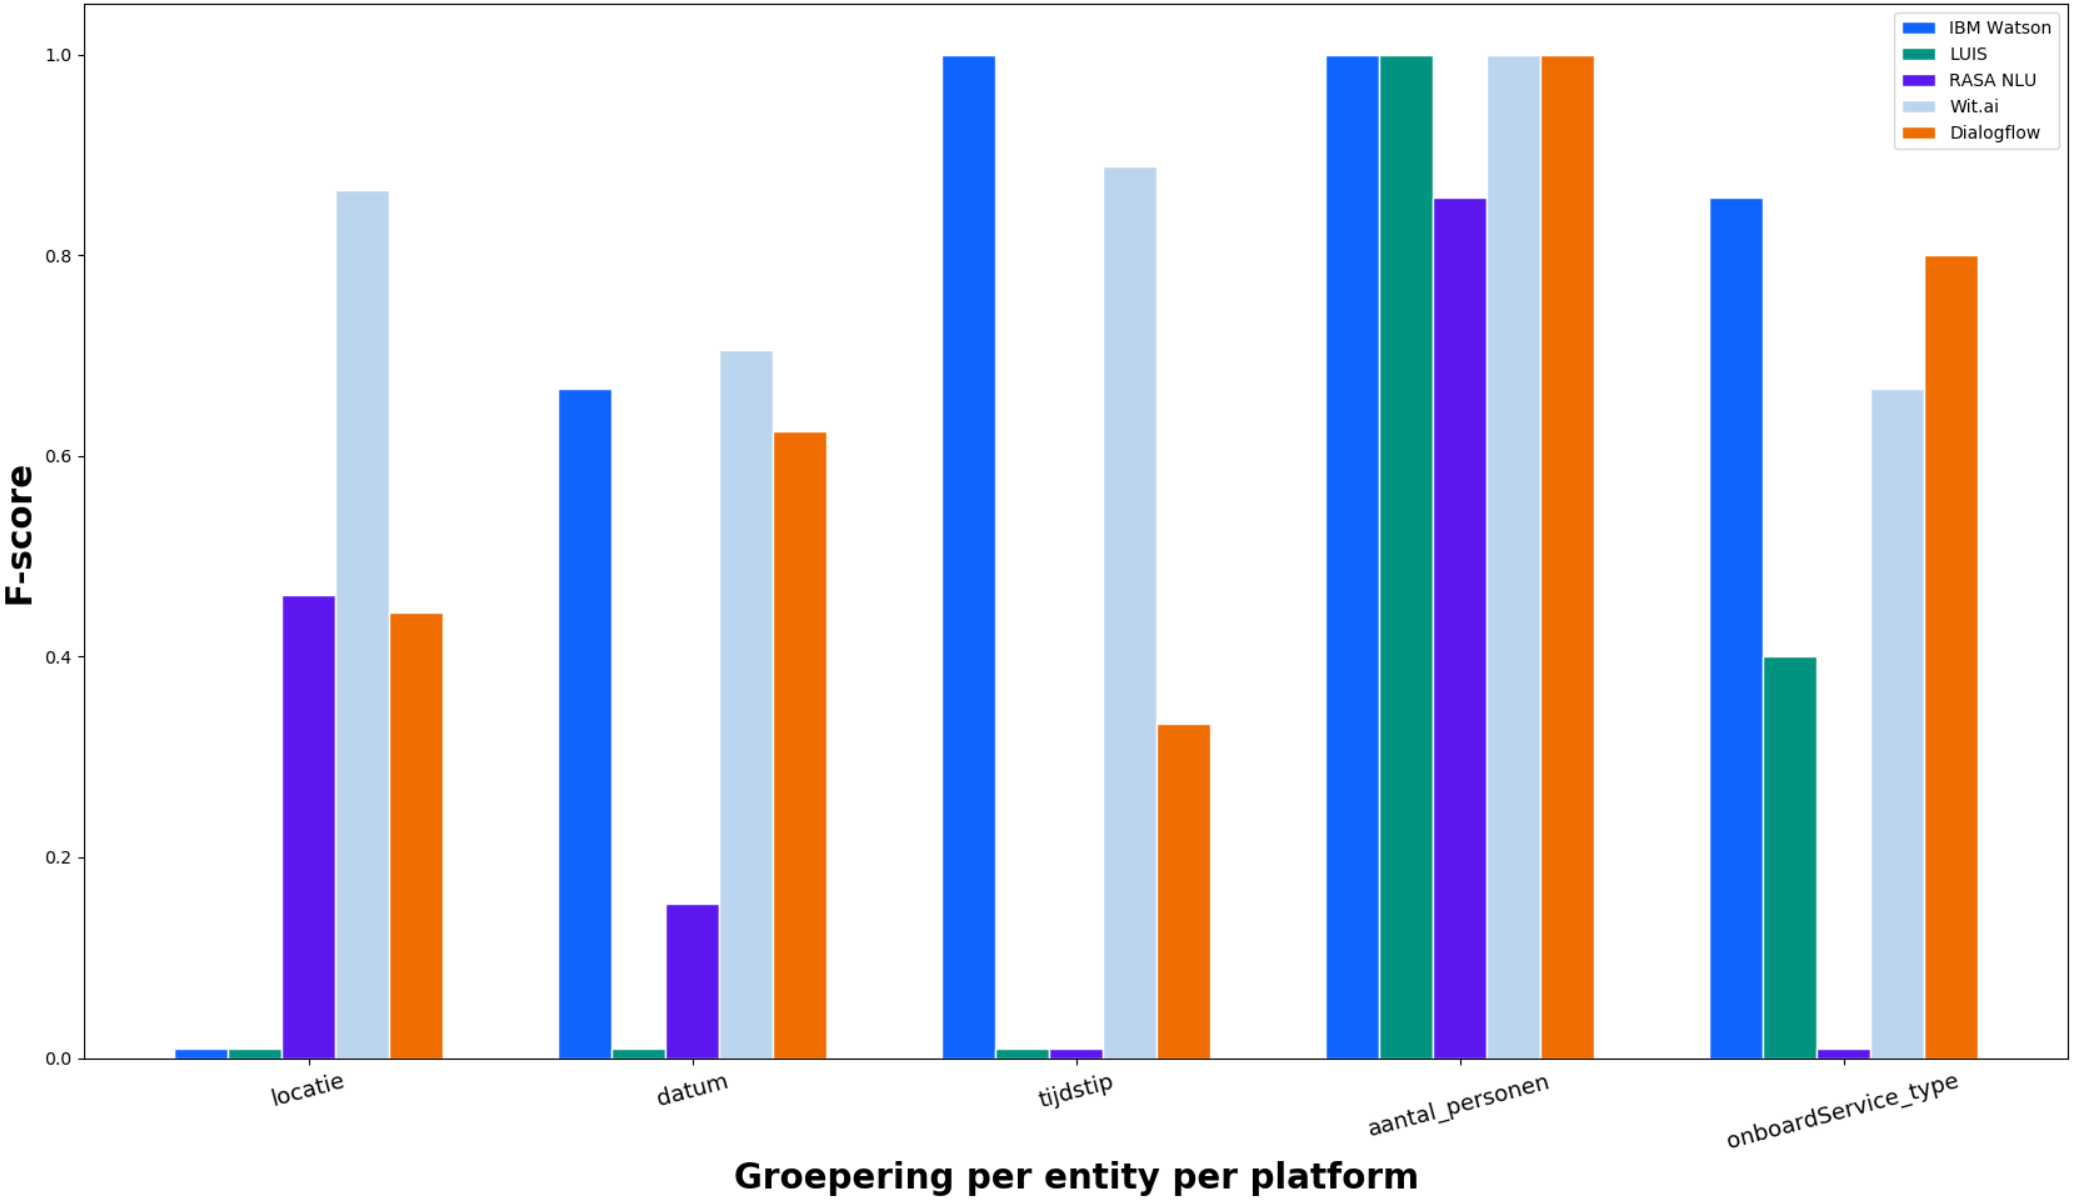
\includegraphics[width=\textwidth]{chart-entity-spelling}
    \caption{Grafiek die de F-scores per entity per platform visualiseert bij het gebruik van spellingsfouten}
\end{figure}














